\subsubsection[Measurements in \ttH and \tH production modes]{Measurements in \ttH and \tH production modes\footnote{Contacts editors: A. Calandri, M. Schr\"oder}}


One of the main targets of the High-Luminosity LHC upgrade is to achieve precision measurements of the Higgs boson properties.
The Yukawa coupling of the Higgs boson to the top quark is expected to be of the order of unity and could be partially sensitive to effects beyond the Standard Model.
Therefore, a direct measurement of the coupling of the Higgs boson to top quarks is extremely important to access possible deviations in the top quark's Yukawa couplings due to couplings to new particles.
Such a measurement can be performed by measuring the rate of the process where the Higgs boson is produced in association with a pair of top quarks (\ttH) or a single top quark (\tH).
Even though the \ttH process is characterised by a small cross section compared to the dominant gluon fusion Higgs boson production (approximately two orders of magnitude smaller), the signature with top quarks in the final state can be exploited to reconstruct the event and gives access to many Higgs boson decay modes.
The SM \tH production cross-section is yet smaller by a factor five, but due to interference effects between diagrams with top-Higgs and W-boson-Higgs couplings, the process allows access to the sign of the top-Higgs Yukawa coupling.
The ATLAS and CMS Collaborations have searched for the \ttH and \tH production with LHC Run 2 data of 2015, 2016, and 2017, and observed the Higgs boson production in association with a top-quark pair~\cite{Aaboud:2018urx,Sirunyan:2018hoz}.
The analyses are sensitive to a large variety of final-state event topologies, H$\rightarrow$WW$^{*}$, H$\rightarrow$ZZ$^{*}$, H$\rightarrow \tau^{+}\tau^{-}$, \Htobb and H$\rightarrow \gamma\gamma$.
Dedicated multivariate analysis techniques, including boosted decision trees and deep neural networks, that combine the information of several discriminating variables, as well as classifiers based on a matrix element method are utilised to identify the signal against the background.

In this Section, projections based on dedicated analyses with 36\fbinv of Run-II data of 2016 are presented, which target the \ttH, \Htobb channel with leptonic decays of the \ttbar system~\cite{Aaboud:2017rss,Sirunyan:2018mvw} and the \ttH multi-lepton final state~\cite{Aaboud:2017jvq}, where the Higgs boson decays into a pair of Z and W vector bosons or into $\tau$ leptons.
Furthermore, results are presented for the projection of a search for \tH production that considers all of the above decay channels~\cite{Sirunyan:2018lzm}.


\subsubsubsection{Sensitivity to \ttH production in the \bbbar and multi-lepton final states}

The \ttH analyses in the \Htobb final state benefit from the large branching ratio.
At the same time, the relatively poor b jet energy resolution, the large jet combinatorics, and the sizeable background of SM processes with large modelling uncertainties, in particular \ttbar+heavy-flavour jet (\ttHF) production, pose major challenges.
The expected relative precision of the \ttH, \Htobb cross-section measurement reaches the level of 20\%-14\% for the ATLAS analysis and 15\%-11\% for the CMS analysis ~\cite{ATLAS-PHYS-PUB-2018-XY,CMS-PAS-FTR-18-011} corresponding to 7\%-11\% relative uncertainty on the signal strength ($\mu$), depending on the scenario and the assumptions of the \ttHF background modelling, as detailed below.

Table~\ref{tab:tthbb:breakdown:cms} shows a breakdown of the contributing sources of uncertainty in the CMS analysis; their evolution with integrated luminosity is depicted in Fig.~\ref{fig:tthbb:evolution:cms}.
Compared to the result at 35.9\fbinv, the relative contribution of the experimental uncertainties, such as the b-tagging uncertainty, remains approximately the same, while the signal-theory uncertainty component increases and becomes the major uncertainty component, mostly driven by the inclusive cross-section uncertainty on the SM prediction entering $\mu$.
The statistical uncertainty becomes small compared to the systematic components.
A similar behaviour is observed in the ATLAS analysis.
\begin{table}
  \centering
  \caption{
    Breakdown of the contributions to the expected uncertainties on the \ttH signal-strength $\mu$ in the \Htobb channel at different luminosities for the scenarios S1 and S2 at CMS.
    The uncertainties are given in percent relative to $\mu=1$.
    Results with 35.9\fbinv are intended for comparison with the projections to higher luminosities and differ in parts from~\cite{Sirunyan:2018mvw} for consistency with the projected results: uncertainties due to the limited number of Monte Carlo statistics have been omitted and the assumptions in S1/S2 on the theory uncertainties are applied.
  }
  \label{tab:tthbb:breakdown:cms}
  \begin{tabular}{l rrr rrr}
    \hline
    & \multicolumn{2}{c}{S1} & \multicolumn{2}{c}{S2} \\
    Source & \multicolumn{1}{c}{35.9\fbinv} & \multicolumn{1}{c}{3000\fbinv} & \multicolumn{1}{c}{35.9\fbinv} & \multicolumn{1}{c}{3000\fbinv} \\
    \hline
    Total            & 48.7 &11.1 & 46.1 & 7.3 \\
    Stat             & 26.7 & 2.9 & 26.7 & 2.9 \\
    SigTh            & 10.8 & 8.7 &  5.0 & 4.4 \\
    BkgTh            & 28.6 & 4.1 & 25.6 & 3.5 \\
    ~~~\ttHF XS      & 14.6 & 0.8 & 16.5 & 0.7 \\
    Exp              & 17.4 & 4.2 & 16.6 & 2.6 \\
    ~~~Luminosity    &  1.6 & 1.8 &  0.5 & 0.8 \\
    ~~~B tagging     & 12.0 & 2.8 & 10.8 & 1.6 \\
    ~~~JES           & 10.9 & 1.6 & 11.3 & 1.6 \\
    \hline
  \end{tabular}
\end{table}

\begin{figure}
  \centering
  \begin{tabular}{@{}c@{}c@{}}
    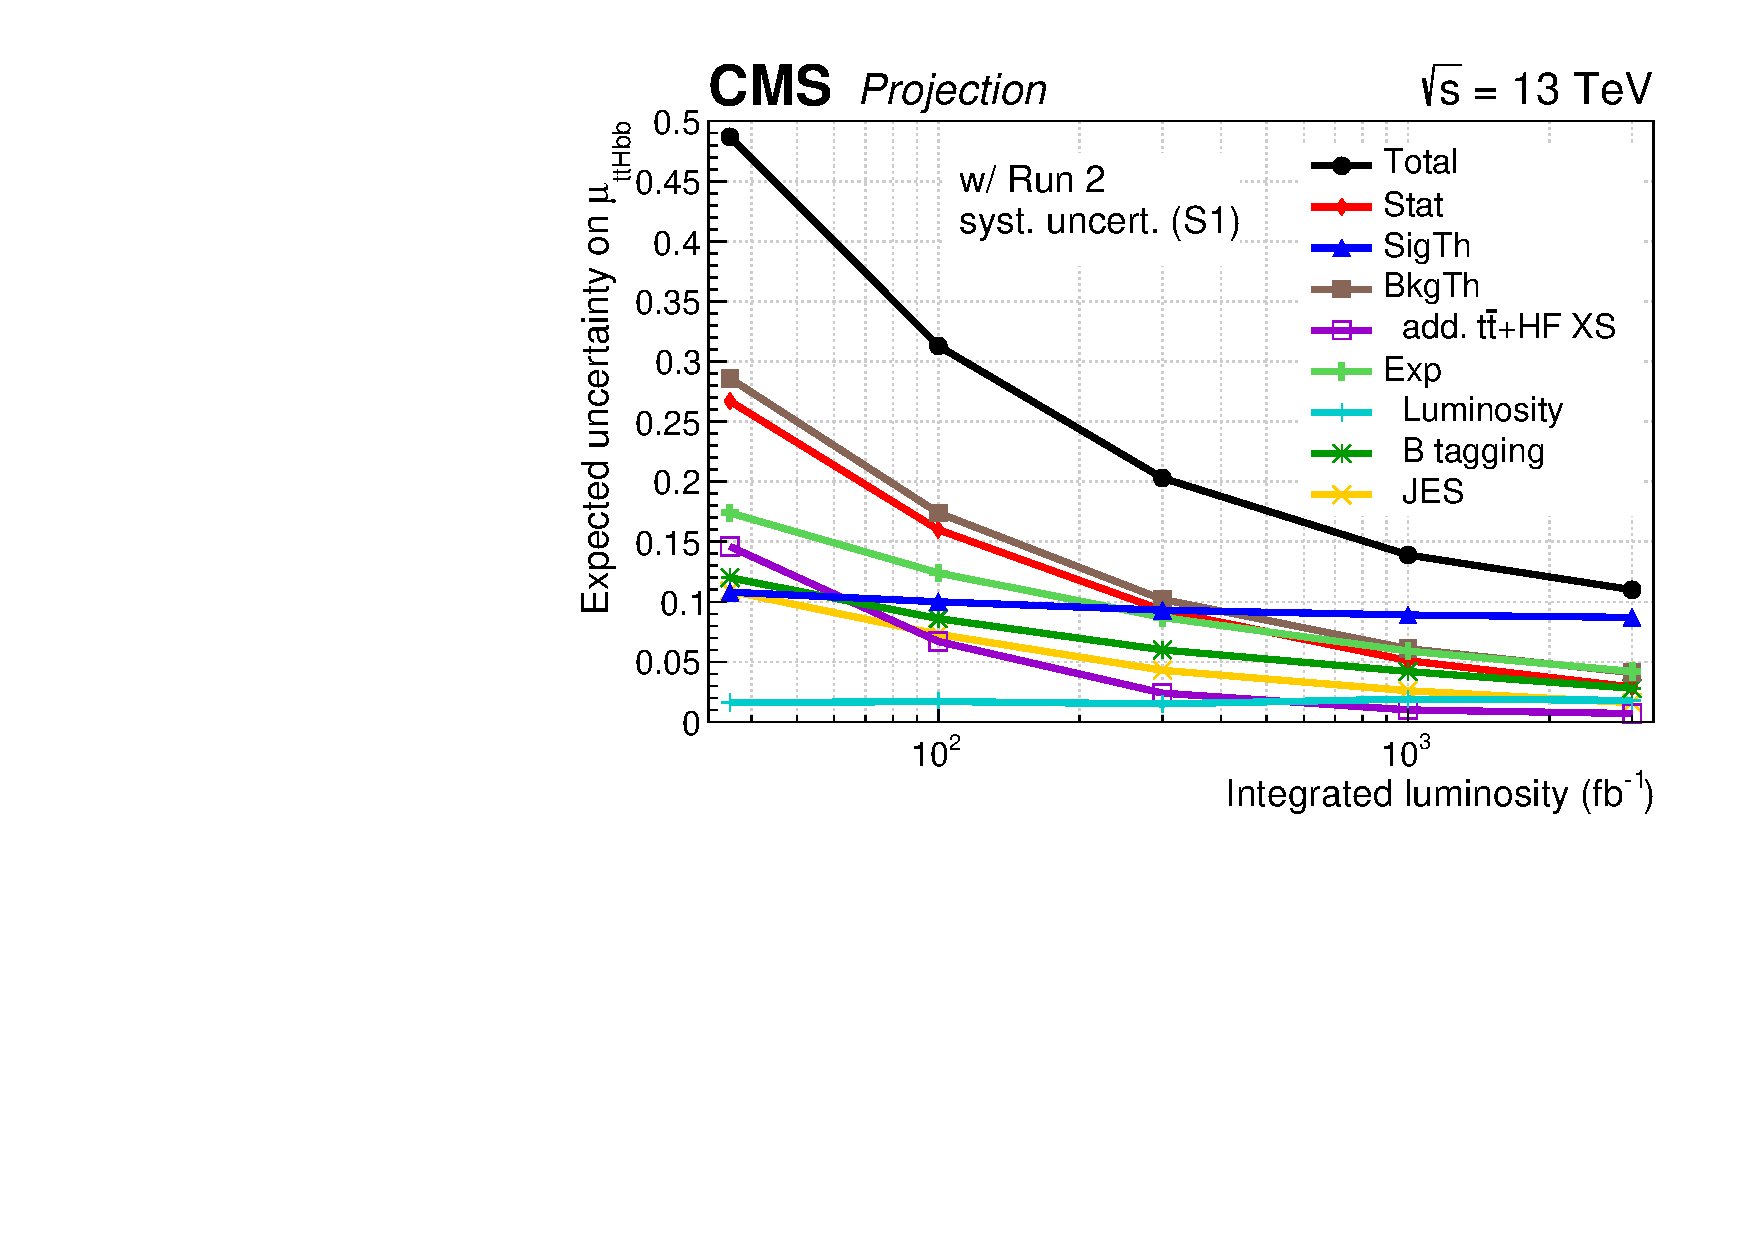
\includegraphics[width=0.49\textwidth]{\main/section2/plots/r_uncertainty_evolution_substracted_YR2018_S1_breakdown_mu_uncertainties_vs_lumi_add_points.pdf} &
    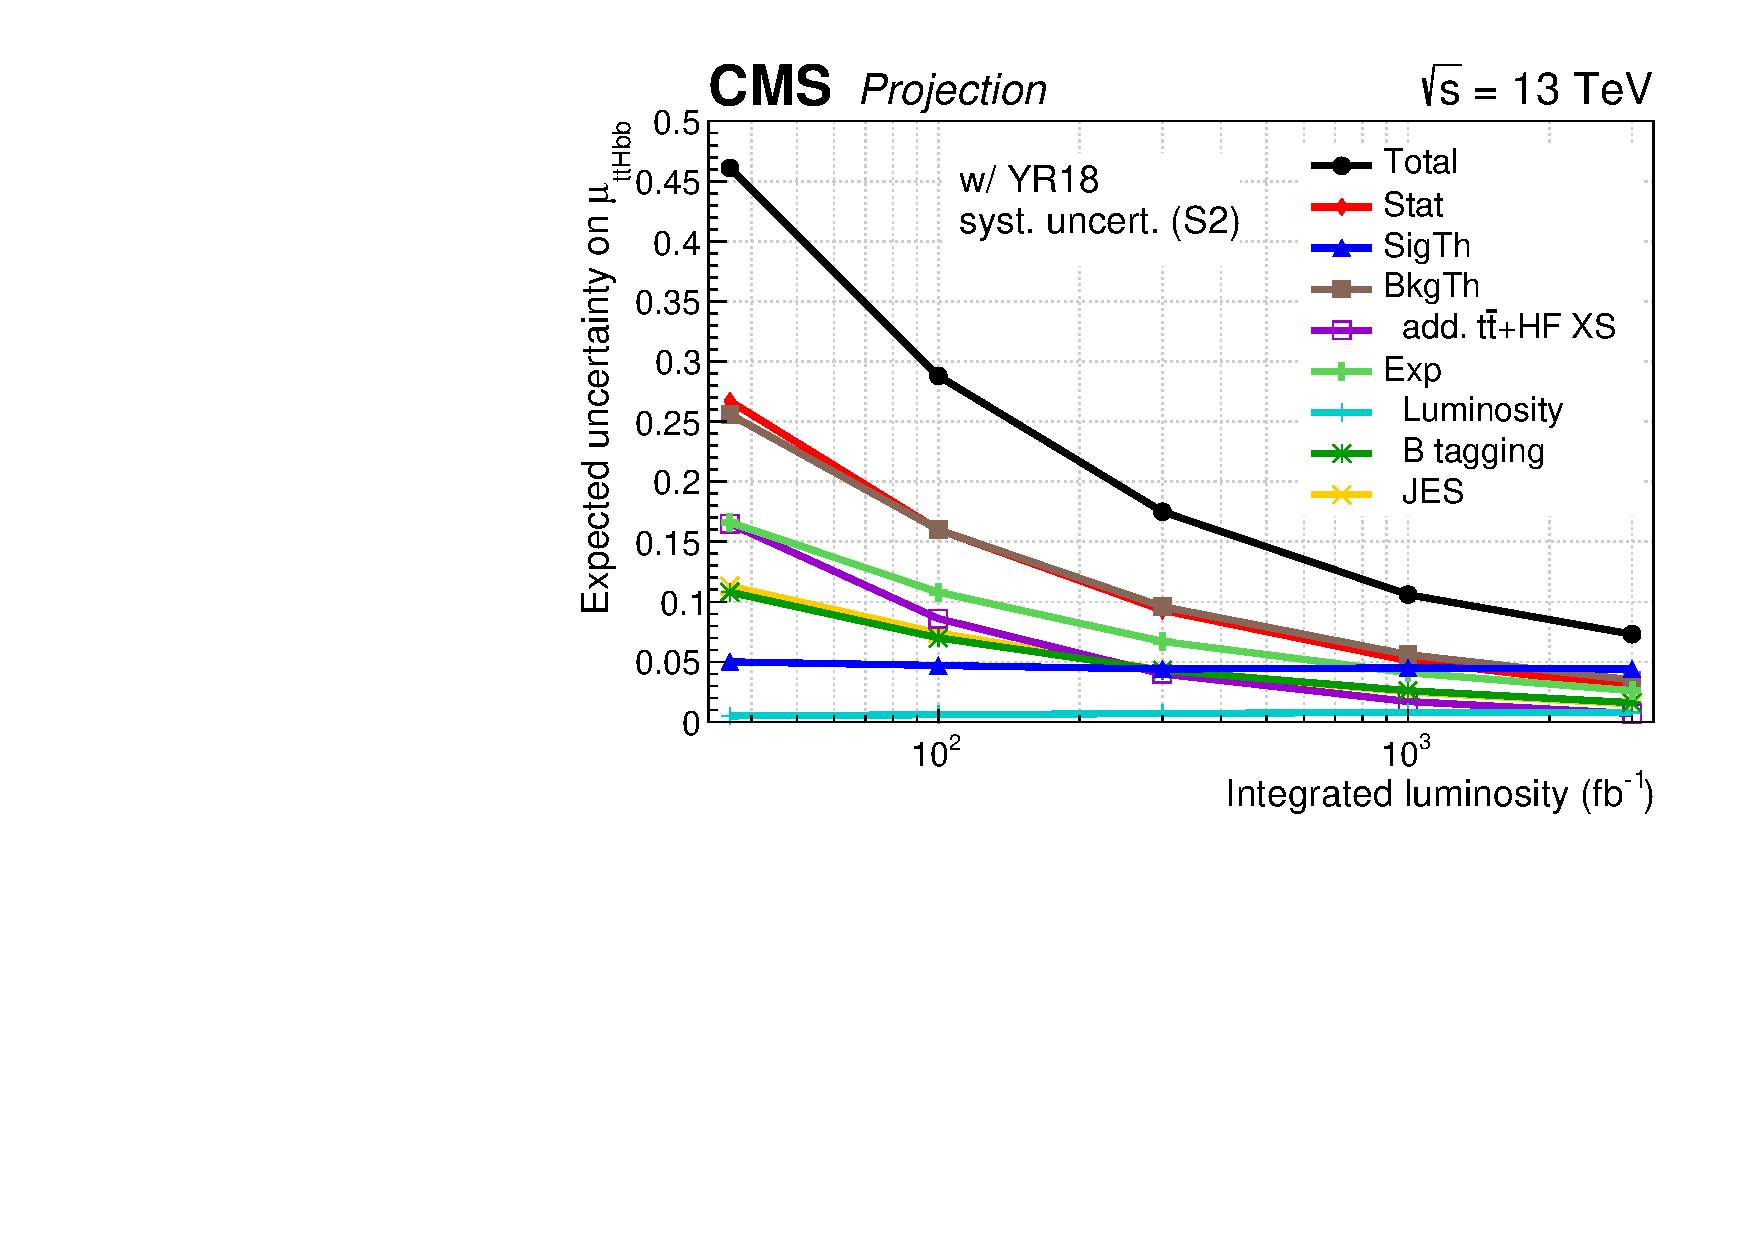
\includegraphics[width=0.49\textwidth]{\main/section2/plots/r_uncertainty_evolution_substracted_YR2018_S2_breakdown_mu_uncertainties_vs_lumi_add_points.pdf} \\
  \end{tabular}
  \caption{
    Expected uncertainties on the \ttH signal strength in the \Htobb channel as a function of the integrated luminosity under the S1 (left) and S2 (right) scenarios at CMS.
    Shown are the total uncertainty (black) and contributions of different groups of uncertainties.
    Results with 35.9\fbinv are intended for comparison with the projections to higher luminosities and differ in parts from~\cite{Sirunyan:2018mvw} for consistency with the projected results: uncertainties due to the limited number of MC events have been omitted and the assumptions in S1/S2 on the theory uncertainties are applied.  
   }
   \label{fig:tthbb:evolution:cms}
\end{figure}

\begin{figure}
  \centering
  \begin{tabular}{@{}c@{}c@{}}
    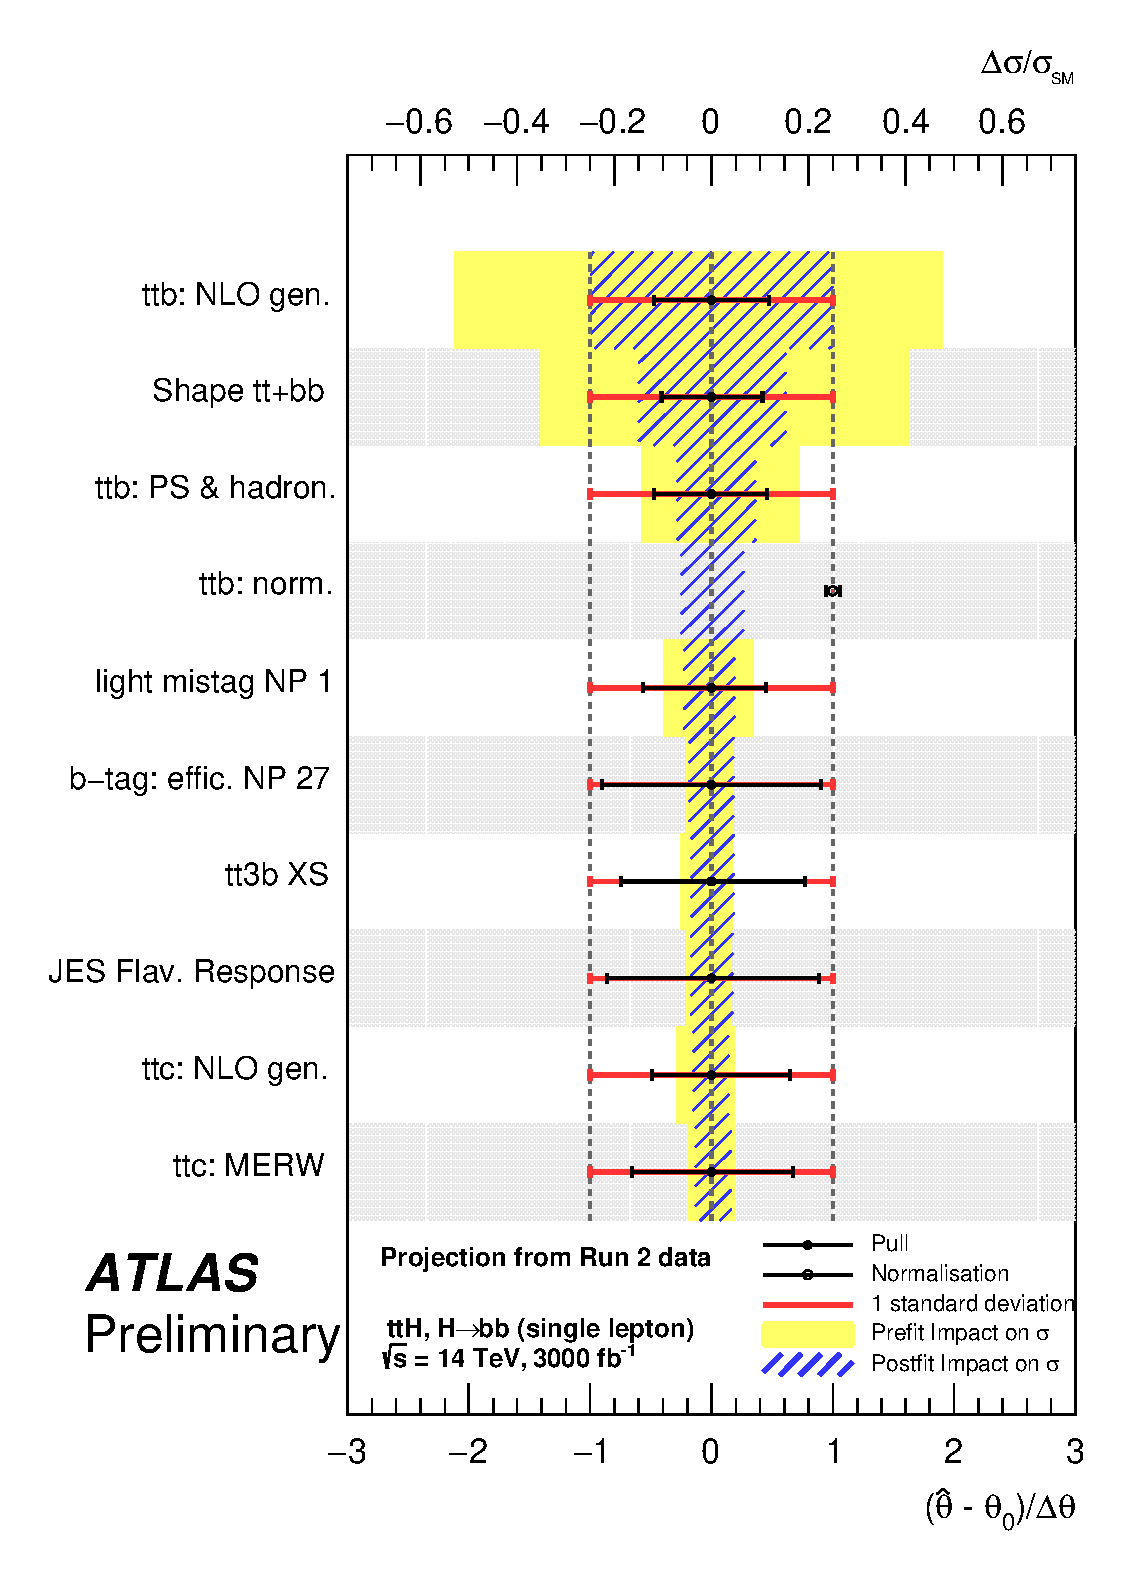
\includegraphics[width=0.49\textwidth]{\main/section2/plots/bblj_XS_postfit} &
    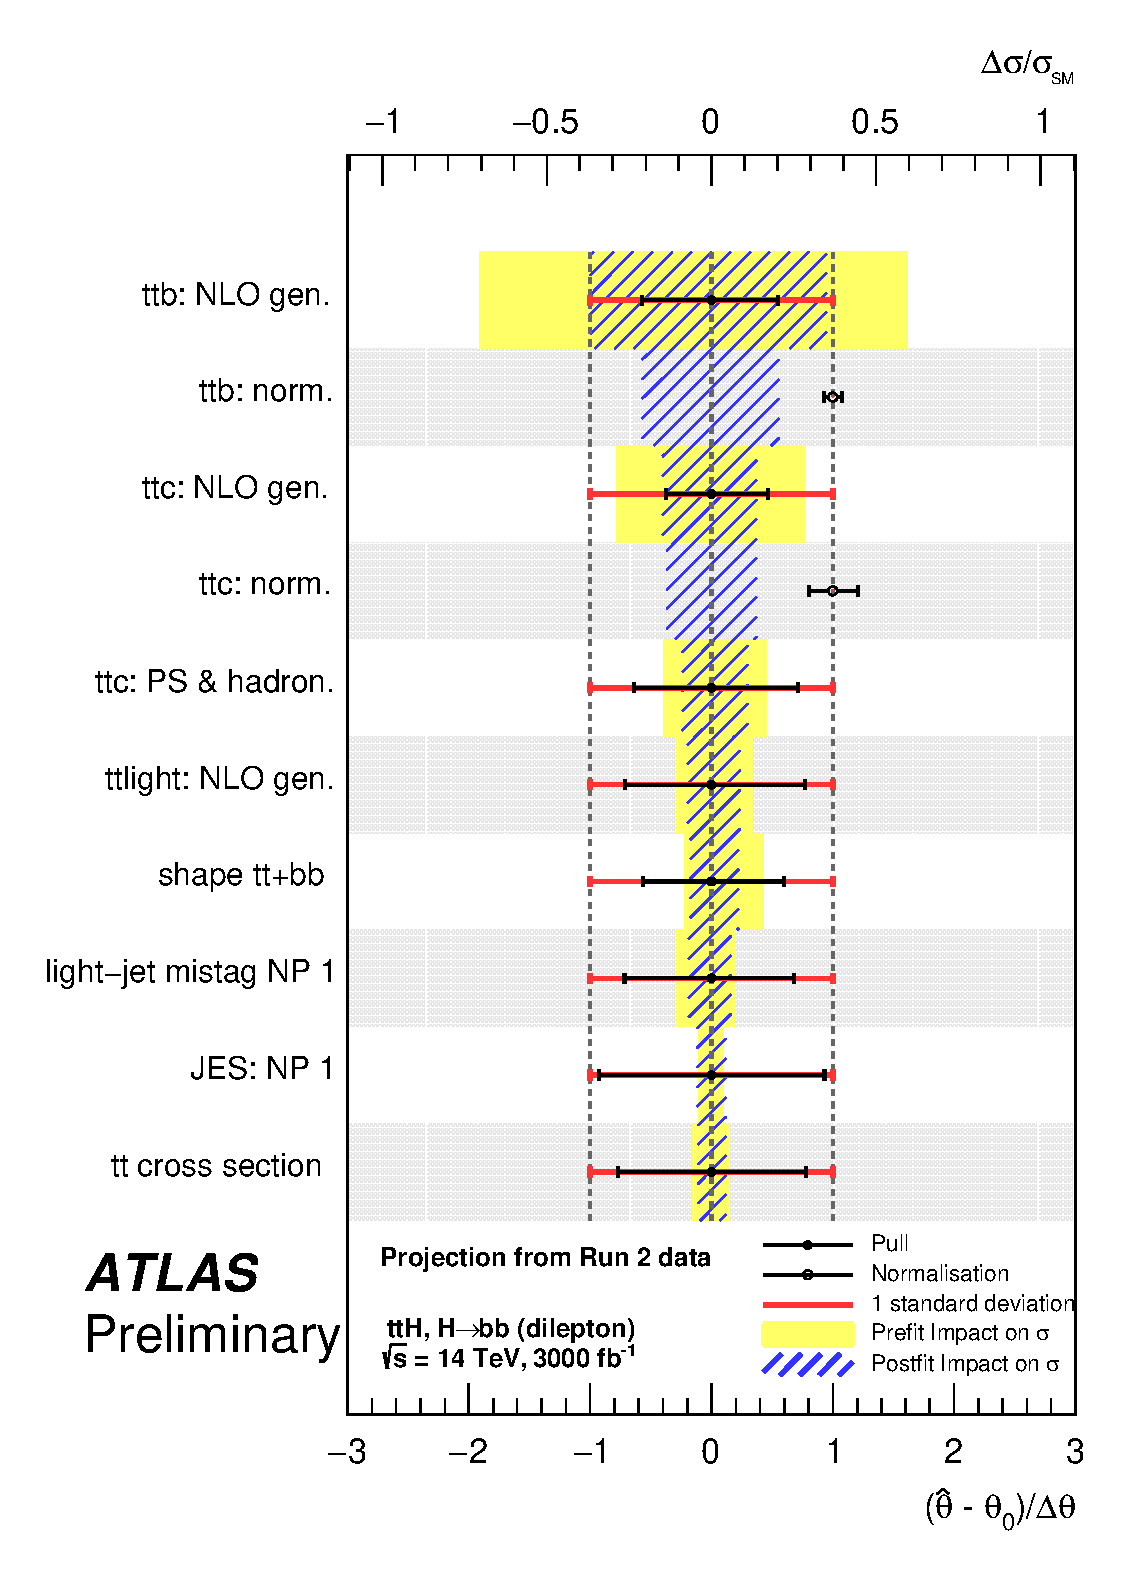
\includegraphics[width=0.49\textwidth]{\main/section2/plots/bbdilep_XS_postfit} \\
  \end{tabular}  
  \caption{
    Ranking of the ten most significant systematics uncertainties under S2 in the single lepton (a) and di-lepton (b) final states at ATLAS listed in accordance to their post-fit impact on the \ttH cross section.
  }
  \label{fig:tthbb:impacts:atlas}
%add ATLAS ranking
\end{figure}

In both analyses, a rather sizeable reduction of the uncertainties related to the modelling of the \ttHF background, which relies on MC simulation, is observed.
Relevant nuisance parameters are constrained to a few percent, such as the nuisance parameters describing the difference between four and five-flavour scheme calculations which is treated as a 2-point systematic uncertainty in the ATLAS analysis (Fig.~\ref{fig:tthbb:impacts:atlas}) or the nuisance parameters describing the additional \ttHF cross-section uncertainties in the CMS analysis (Table~\ref{tab:tthbb:breakdown:cms} and Fig.~\ref{fig:tthbb:evolution:cms}).
This is attributed to the increasing power of the profile likelihood fit to constrain the uncertainties.
%The presented results rely on the \ttHF background model that has been designed for the analyses of 35.9\fbinv of data and that is not expected to work optimally without substantial modifications for higher integrated luminosities.

The results illustrate that the background modelling, which has been designed to work well with 35.9\fbinv of data, will need to be refined at 3000\fbinv, requiring improved simulations or in-situ measurements of the \ttHF processes themselves.
The observed constraints on the \ttHF background model systematics uncertainties shown in Fig.~\ref{fig:tthbb:impacts:atlas} demonstrate that there will be enough data at the HL-LHC to obtain further information about the background beyond the current modelling. The level at which the nuisance parameters are constrained at 3000\fbinv, corresponding to a few percent cross-section uncertainty, demonstrate the level of sensitivity at which the data will be able to distinguish different models and sets a benchmark for the required precision.
Monte Carlo prediction will thus need to improve sufficiently to match the data within the uncertainties expected at 3000\fbinv.
%The results presented here have to be interpreted in light of these considerations.

Following the expected improvement by a factor two to three in the theoretical uncertainties on the \ttHF cross-section calculation described in Section~\ref{sec:hl-lhc-ttH}, ATLAS and CMS have also performed the \ttH, \Htobb extrapolation assuming that the reduction of the \ttHF modelling uncertainties is limited to factors of two (in scenario S1) and three (in scenario S2) relative to the uncertainty at 35.9\fbinv.
In this case, the obtained relative \ttHF modelling uncertainties are approximately 23\% (S1) and 15\% (S2) in the ATLAS analysis as reported in Table~\ref{tab:tthbb:breakdown:atlas} and approximately 15\% (S1) and 10\% (S2) in the CMS analysis. These results enter the combined coupling measurement presented in Sections~\ref{sec2:exp_combination} and~\ref{sec2:exp_kappa}. The impact of limiting the constraints of the \ttHF uncertainties on the total uncertainties on the extracted parameters is relatively small, e.g.\ the uncertainty on $\kappa_{\text{t}}$ increases by approximately 10\% and 15\% in CMS and ATLAS, respectively. 
\begin{table}
  \centering\small
\renewcommand{\arraystretch}{1.3}
  \begin{tabular}{c|c|c|cccc|c}
    \hline \hline
    Final state & Scenario & $\Delta_{\textrm {tot}}/\sigma_{\textrm {SM}}$ & $\Delta_{\textrm {stat}}/\sigma_{\textrm {SM}}$ & $\Delta_{\textrm {exp}}/\sigma_{\textrm {SM}}$ & $\Delta_{\textrm {sig}}/\sigma_{\textrm {SM}}$ & $\Delta_{\textrm {bkg}}/\sigma_{\textrm {SM}}$
 & $\Delta\mu_{\textrm {sig}}$ \\
    \hline
    $t\bar{t} H,H \rightarrow$ $b\bar{b}$ & Run 2, 36~\ifb  & $^{+0.61}_{-0.61}$ & $^{+0.22}_{-0.22}$ & $^{+0.27}_{-0.28}$ & $^{+0.10}_{-0.09}$ & $^{+0.47}_{-0.47}$ & $^{+0.15}_{-0.15}$ \\
    (single lepton) & HL-LHC S1   & $^{+0.25}_{-0.20}$      & $^{+0.02}_{-0.02}$     & $^{+0.10}_{-0.10}$      & $^{+0.08}_{-0.06}$ &  $^{+0.22}_{-0.17}$ & $^{+0.10}_{-0.11}$ \\
    & HL-LHC S2  & $^{+0.18}_{-0.15}$      & $^{+0.02}_{-0.02}$     & $^{+0.09}_{-0.09}$      & $^{+0.06}_{-0.05}$ &$^{+0.14}_{-0.11}$  & $^{+0.08}_{-0.07}$ \\
    \hline
    $t\bar{t} H,H \rightarrow$ $b\bar{b}$   & Run 2, 36~\ifb  & $^{+1.06}_{-1.08}$ & $^{+0.51}_{-0.51}$ & $^{+0.32}_{-0.31}$ & $^{+0.11}_{-0.12}$ & $^{+0.90}_{-0.92}$  & $^{+0.14}_{-0.14}$ \\
  (di-lepton) & HL-LHC S1             & $^{+0.32}_{-0.26}$      & $^{+0.06}_{-0.06}$      & $^{+0.13}_{-0.13}$      & $^{+0.08}_{-0.07}$ & $^{+0.27}_{-0.21}$  & $^{+0.11}_{-0.09}$ \\
    & HL-LHC  S2               & $^{+0.23}_{-0.20}$      & $^{+0.06}_{-0.06}$     & $^{+0.11}_{-0.11}$      & $^{+0.06}_{-0.06}$ & $^{+0.17}_{-0.15}$ & $^{+0.08}_{-0.08}$ \\
    \hline\hline
\end{tabular}  
  \caption{
    Breakdown of the contributions to the expected uncertainties on the \ttH cross section in the \Htobb channel at different luminosities for the scenarios S1 and S2 at ATLAS. As discussed in the text, the extrapolation assumes the limitations on the reduction of the \ttHF modelling to a factor 2 and a factor 3 of the Run 2 prior uncertainties (Section \ref{sec:hl-lhc-ttH}).
    Therefore, the additional modelling uncertainty used for the extrapolation is 23\% in S1 and 15\% in S2.
    Uncertainties due to the limited number of Monte Carlo statistics have been omitted and the assumptions in S1/S2 on the theory uncertainties are applied.  
  }
  \label{tab:tthbb:breakdown:atlas}
  % add ATLAS numbers
\end{table}

In conclusion, \ttH production in the \Htobb final state will provide a powerful channel to probe the top-Higgs Yukawa coupling at the HL-LHC.
The control of the \ttHF background is crucial, and it is expected to benefit from measuring relevant quantities from data, thus mitigating the impact of theoretical uncertainties.

ATLAS performs the extrapolation to HL-LHC also for the ttH multi-lepton (ML) final state~\cite{ATLAS-PHYS-PUB-2018-XY} where the Higgs boson decays into a pair of Z and W vector bosons or into a pair of $\tau$ leptons. Table \ref{tab:tthml:breakdown:atlas} shows the results on the extrapolation to 3000 fb$^{-1}$ under S1 and S2. As shown in the ranking plot in Figure \ref{fig:tthml:impacts:atlas}, in the $\tau$ final state, the dominant uncertainty pertains to the object reconstruction for such a channel. It is also worth noting that the main theoretical systematic uncertainties concerns the modelling of the tt+V background. Finally, fake lepton uncertainties are moderately constrained as well: this is due to the absence of a reduction factor of prior uncertainties for such a source of systematic uncertainties under S1 and S2. 
\begin{table}
  \centering\small
  \renewcommand{\arraystretch}{1.3}
  \begin{tabular}{c|c|c|cccc|c}
    \hline \hline
    Final state & Scenario & $\Delta_{\textrm {tot}}/\sigma_{\textrm {SM}}$ & $\Delta_{\textrm {stat}}/\sigma_{\textrm {SM}}$ & $\Delta_{\textrm {exp}}/\sigma_{\textrm {SM}}$ & $\Delta_{\textrm {sig}}/\sigma_{\textrm {SM}}$ & $\Delta_{\textrm {bkg}}/\sigma_{\textrm {SM}}$
 & $\Delta\mu_{\textrm {sig}}$ \\
    \hline
    $t\bar{t} H,H \rightarrow$ ML   & Run 2, 36~\ifb & $^{+0.40}_{-0.40}$ & $^{+0.33}_{-0.34}$ & $^{+0.15}_{-0.15}$ & $^{+0.10}_{-0.10}$ & $^{+0.13}_{-0.13}$ & $^{+0.13}_{-0.13}$ \\
    (no $\tau$) & HL-LHC S1 & $^{+0.18}_{-0.18}$ & $^{+0.04}_{-0.04}$ & $^{+0.13}_{-0.14}$ & $^{+0.08}_{-0.08}$ & $^{+0.12}_{-0.12}$ & $^{+0.11}_{-0.11}$ \\
    & HL-LHC S2& $^{+0.17}_{-0.17}$      & $^{+0.04}_{-0.04}$     & $^{+0.12}_{-0.13}$      & $^{+0.05}_{-0.05}$ & $^{+0.09}_{-0.09}$ & $^{+0.07}_{-0.07}$ \\
    \hline
    $t\bar{t} H,H \rightarrow$ ML  & Run 2, 36~\ifb  & $^{+0.64}_{-0.64}$ & $^{+0.54}_{-0.54}$ & $^{+0.29}_{-0.29}$ & $^{+0.10}_{-0.09}$ & $^{+0.14}_{-0.13}$  & $^{+0.13}_{-0.13}$ \\
    (with $\tau$) & HL-LHC S1             & $^{+0.27}_{-0.28}$      & $^{+0.07}_{-0.07}$     & $^{+0.23}_{-0.23}$      & $^{+0.09}_{-0.08}$ & $^{+0.12}_{-0.12}$ & $^{+0.11}_{-0.11}$ \\
    & HL-LHC S2           & $^{+0.25}_{-0.25}$      & $^{+0.07}_{-0.07}$     & $^{+0.22}_{-0.22}$      & $^{+0.05}_{-0.05}$ &  $^{+0.07}_{-0.07}$ & $^{+0.07}_{-0.07}$ \\
    \hline\hline
\end{tabular}  
  \caption{
    Breakdown of the contributions to the expected uncertainties on the \ttH cross section in the multi-lepton channel at different luminosities for the scenarios S1 and S2 at ATLAS. Uncertainties due to the limited number of Monte Carlo statistics have been omitted and the assumptions in S1/S2 on the theory uncertainties are applied.
  }
  \label{tab:tthml:breakdown:atlas}
  % add ATLAS numbers
\end{table}
\begin{figure}
  \centering
    \begin{tabular}{@{}c@{}c@{}}
    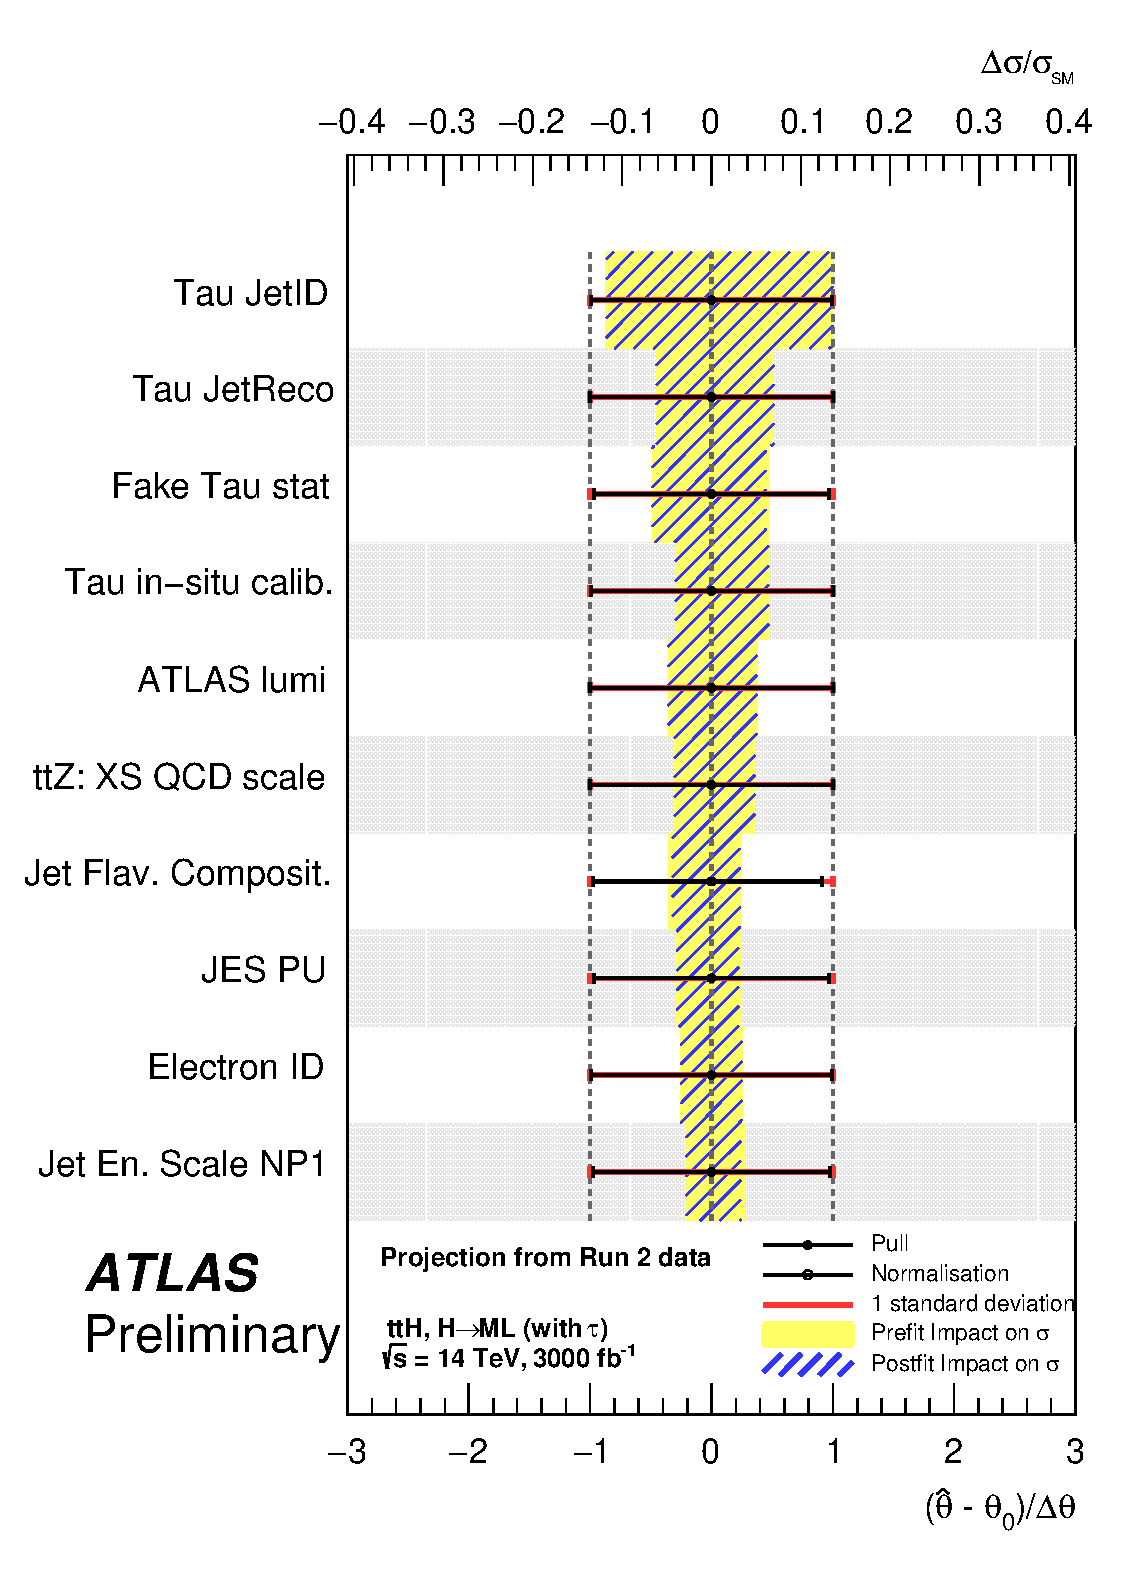
\includegraphics[width=0.49\textwidth]{\main/section2/plots/MLwithTau_XS_postfit} &
    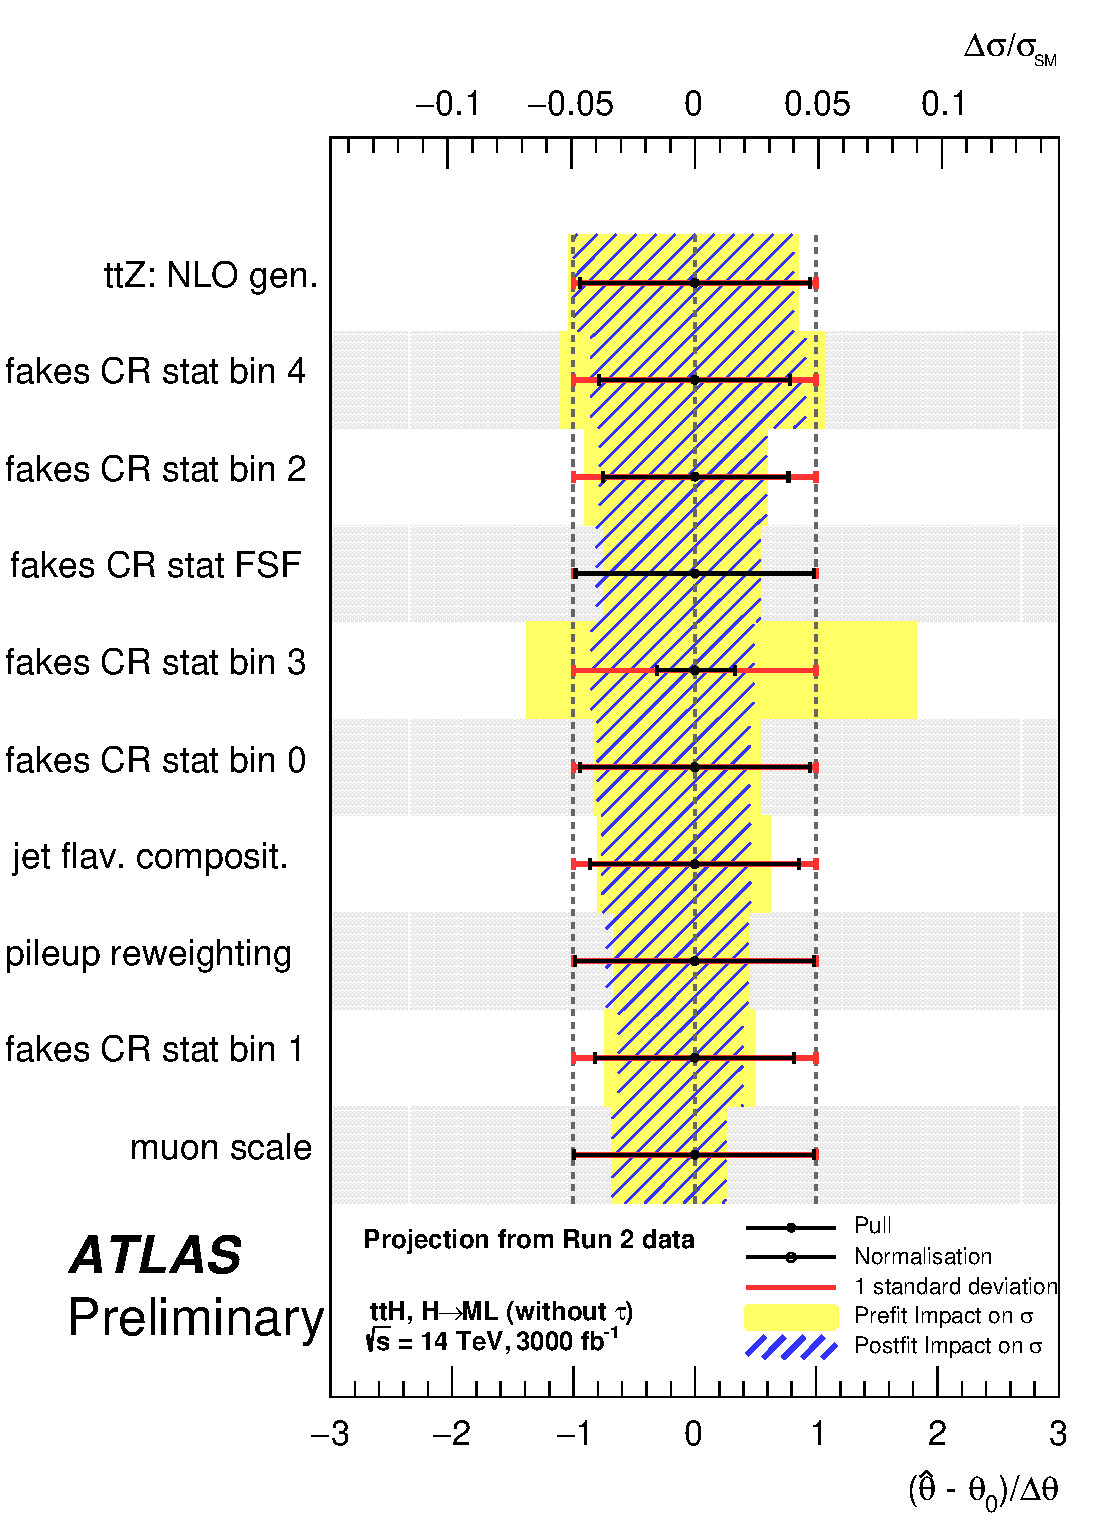
\includegraphics[width=0.49\textwidth]{\main/section2/plots/MLnoTau_XS_postfit} \\
  \end{tabular}  
  \caption{
    Ranking of the ten most significant systematic uncertainties under S2 in the \ttH multi-lepton (ML) final state with (a) and without (b) $\tau$ leptons in the ATLAS analysis listed in accordance to their post-fit impact on the \ttH cross section.
  }
  \label{fig:tthml:impacts:atlas}
 %add ATLAS ranking
\end{figure}


\subsubsubsection{Sensitivity to \tH production}
\footnote{Contacts: K. Mazumdar, P. Das}

The sensitivity to the $\tH$ process at the HL-LHC is determined by extrapolating a combination of Run~2 analyses based on $35.9\fbinv$ of data at $\sqrt{s}= 13 \UTeV$~\cite{Sirunyan:2018lzm}. Two of these analyses are dedicated searches for $\tHq$: one targets a multi-lepton final state in which the Higgs boson decays to $\ww$, $\zz$ or $\tautau$ pairs, and the other targets the $\hbb$ decay. In both analyses the presence of at least one central b tagged jet and an isolated lepton from the top quark decay is required. Furthermore, the presence of a light quark jet at high pseudorapidity, a unique feature of the $\tHq$ production mode, is exploited. Both analyses also rely heavily on multivariate techniques to discriminate the signal against the large $\ttjets$ background. The $\gamma\gamma$ final state is also utilised, via a reinterpretation of the inclusive $\hgg$ analysis~\cite{Sirunyan:2018ouh}. In this analysis the $\mathrm{tHq}$ and $\mathrm{tHW}$ processes primarily contribute to the``$\mathrm{t\bar{t}H}$ leptonic'' and ``$\mathrm{t\bar{t}H}$ hadronic'' event categories, and these are included in the combination.


In Figure~\ref{fig:limit} the variation of the expected upper limits on $\mu_{\tH}$ is shown as a function of the integrated luminosity for the S1 and S2 scenarios. The limits are determined assuming a background-only hypothesis in which the $\tth$ process is considered as following the SM expectation ($\mu_{\tth} = 1$). In order to minimise further assumptions on the rate of $\tth$ production, $\mu_{\tth}$ is treated as a free parameter in the fit.
In the S1 scenario the expected median upper limit on $\mu_{\tH}$ at 3000 \fbinv is determined to be 2.35.
The corresponding value in S2 is 1.51. With the $3000 \fbinv$ dataset and foreseen reduction in systematic uncertainties in S2, the expected upper limit on $\mu_{\tH}$ improves by about a factor of eight with respect to the current exclusion.

\begin{figure}[hbtp]
\begin{center}
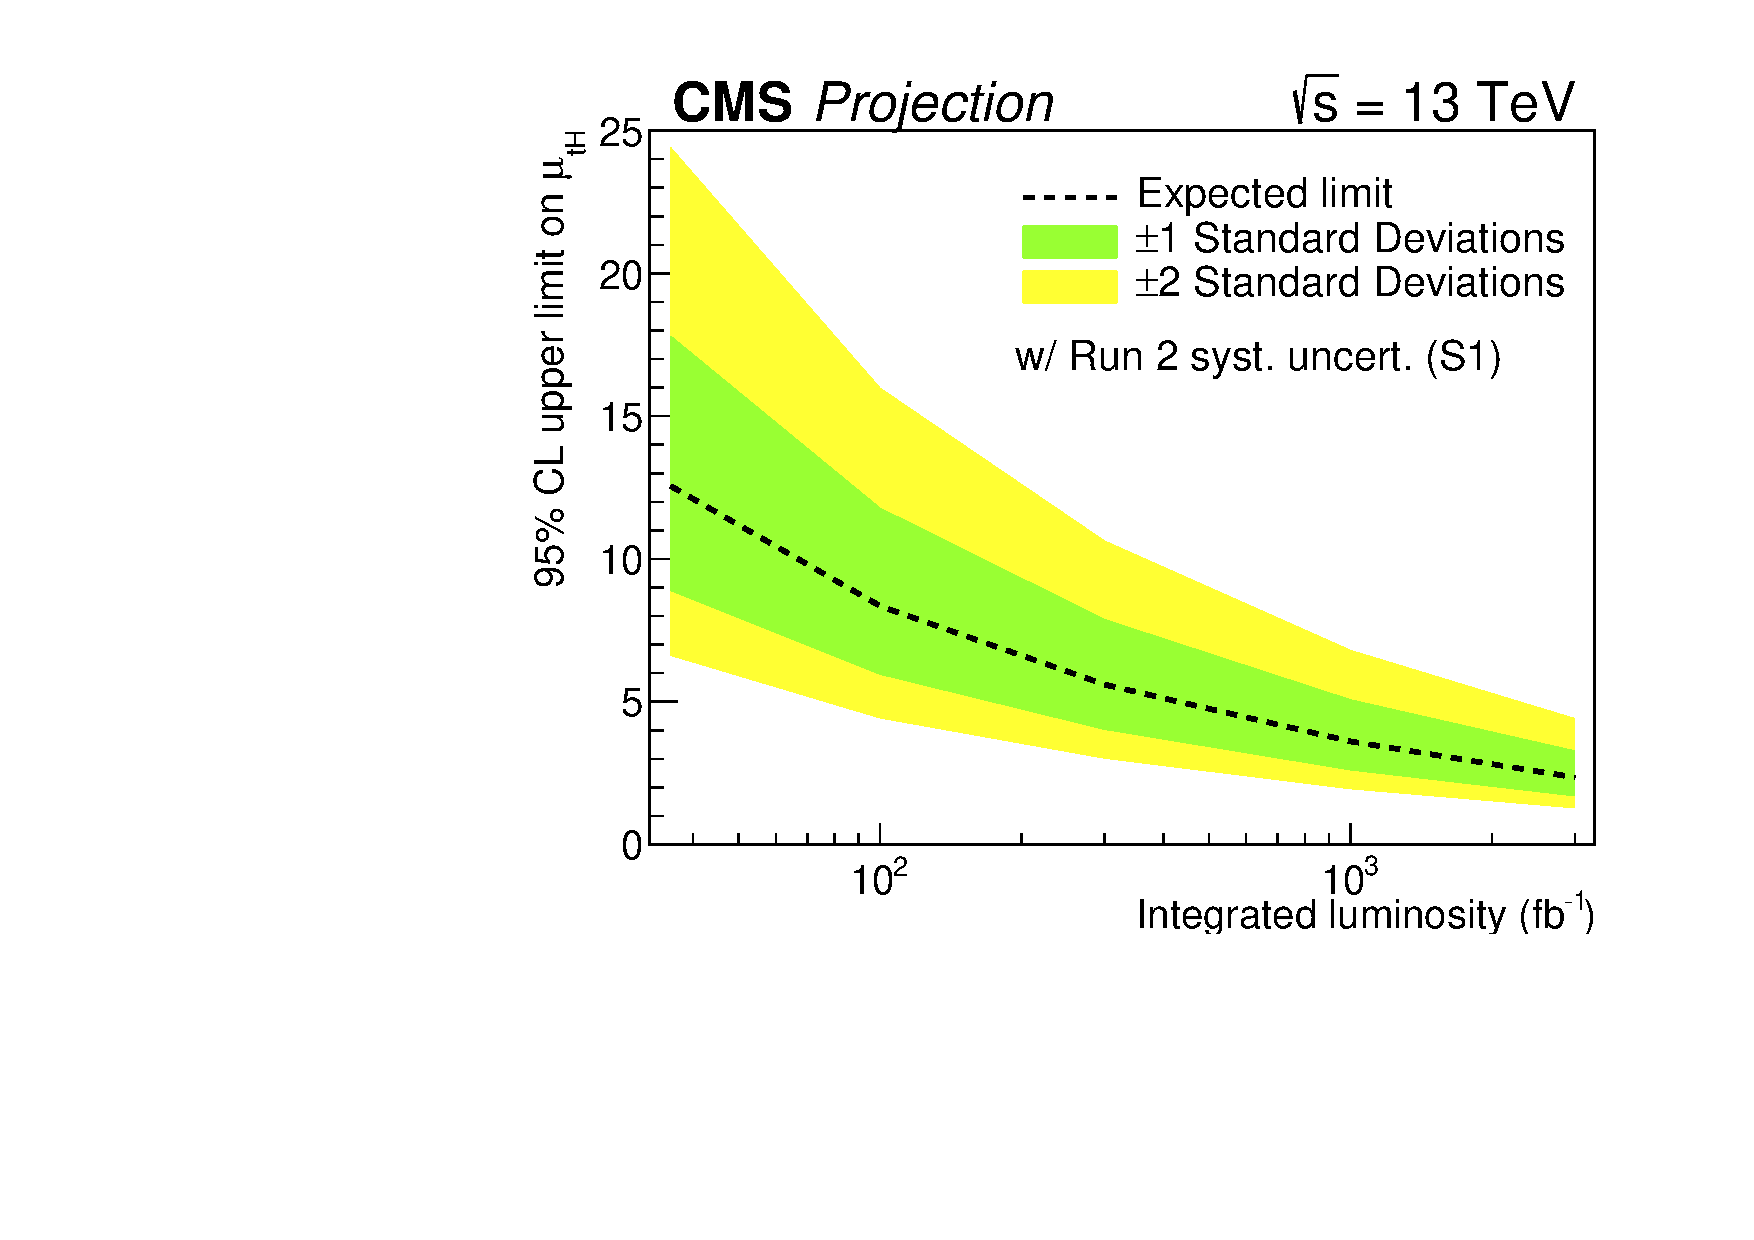
\includegraphics[width=0.45\textwidth]{\main/section2/plots/channels/limits_S1.pdf} \hspace{1cm}
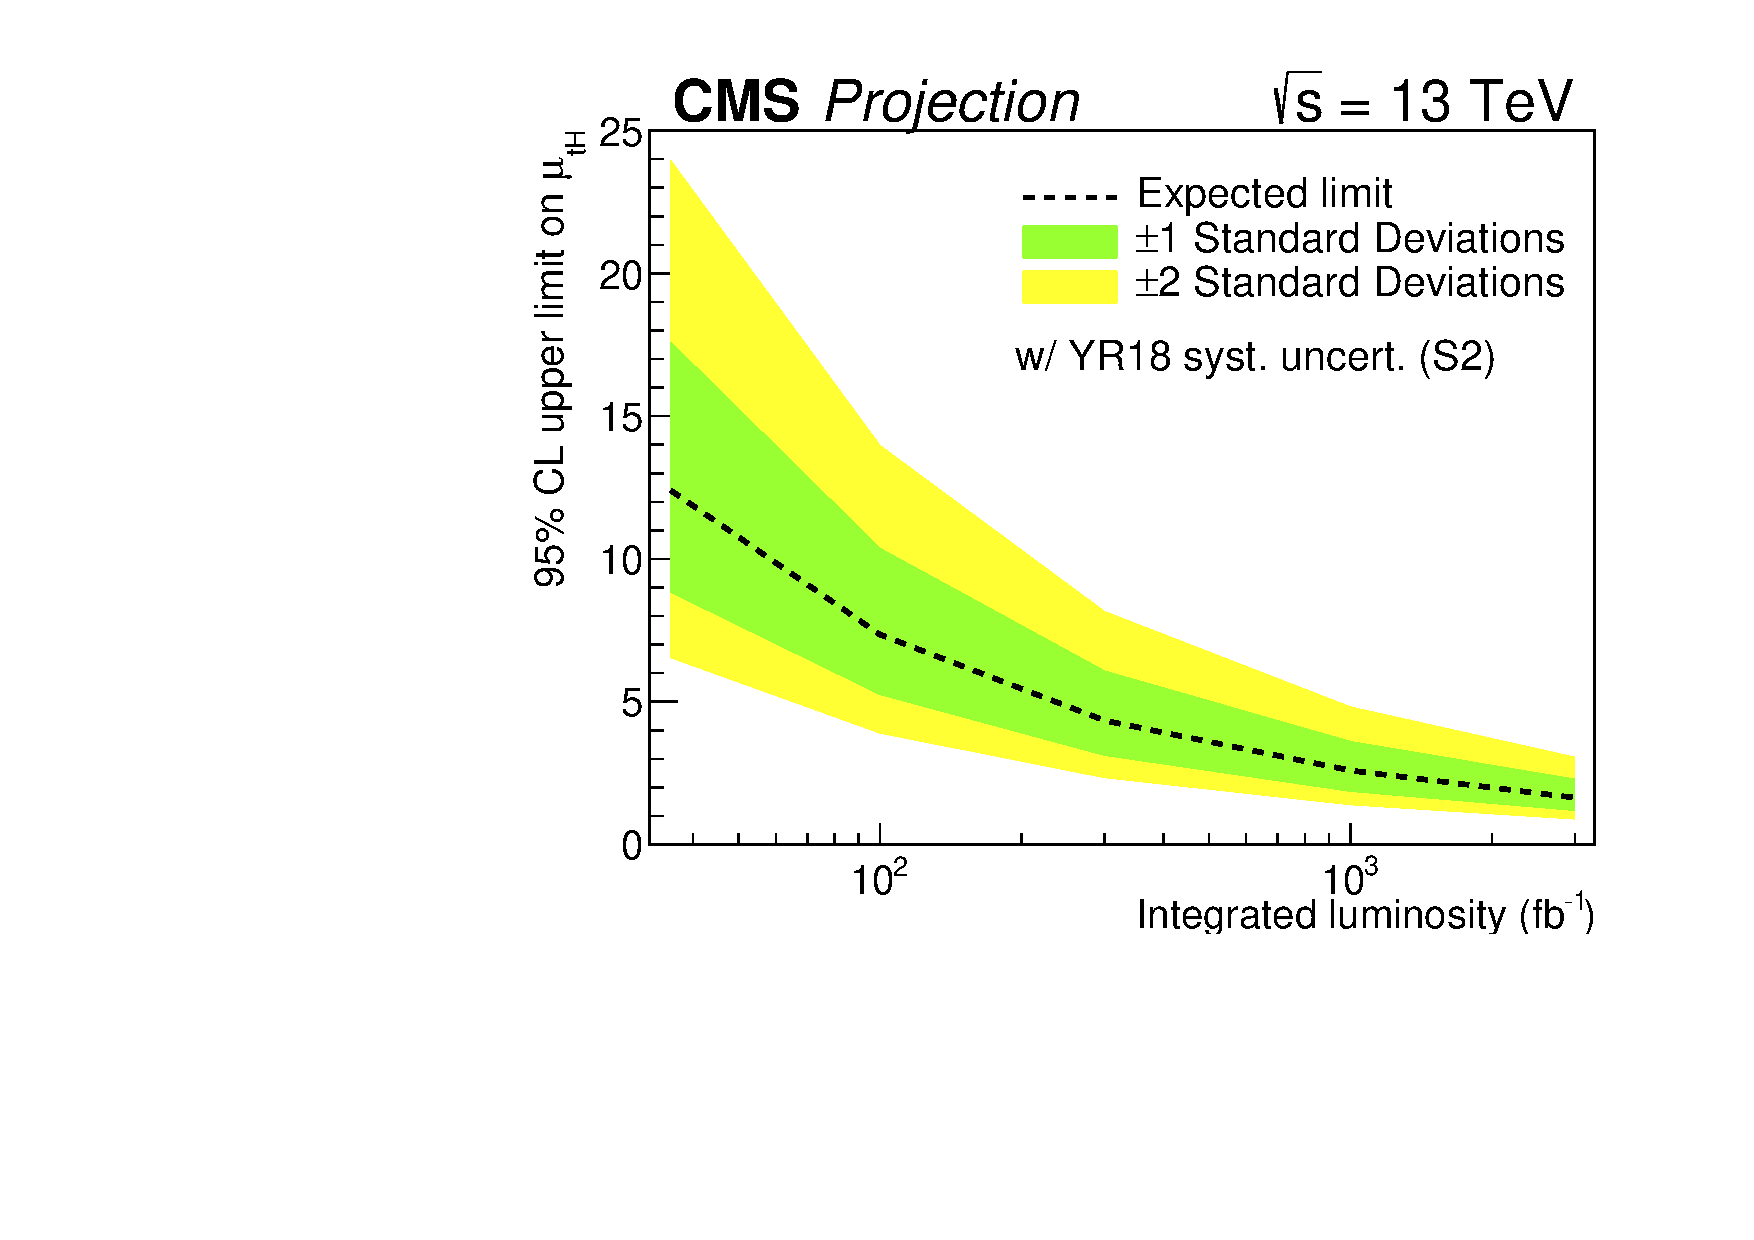
\includegraphics[width=0.45\textwidth]{\main/section2/plots/channels/limits_S2.pdf}
\end{center}
\caption{The variation of expected upper limit on $\mu_{\tH}$ with integrated luminosity for two projection scenarios S1 (with Run~2 systematic uncertainties~\cite{CMS-PAS-HIG-18-009}) and S2 (with YR18 systematic uncertainties).}
\label{fig:limit}
\end{figure}

The evolution of the expected uncertainty on the measurement of $\mu_{\tH}$, assuming the SM rate, is given in Table~\ref{tab:muunc}. Values are given for two cases of background: one in which $\mu_{\tth}$ is unconstrained in the fit, and one in which it is fixed to the SM value of 1. In the latter case the uncertainties are reduced by around $10\%$ at $3000\fbinv$, indicating that a precise simultaneous measurement of the $\tth$ signal strength will be needed to obtain the optimal sensitivity to the $\tH$ channel. In both cases it is found that the reduced systematic uncertainties in S2 improve the precision by up to $30\%$.

\begin{table}[htbp]
\centering
\caption{The $\pm1\sigma$ uncertainties on expected $\mu_{\tH}$=1 for scenarios S1 (with Run~2 systematic uncertainties~\cite{CMS-PAS-HIG-18-009}) and S2 (with YR18 systematic uncertainties) at all three luminosities, considering also the case when $\mu_{\ttH}$ is fixed at the SM value 1.} \label{tab:muunc}
\begin{tabular}{@{} l c c@{\hskip 0.15in} c c }
 \hline
  &  & $\mu_{\tth}$ floating & $\mu_{\tth}$ fixed \\
  \hline
\multirow{3}{*}{S1} & 35.9 \fbinv  & ${}_{-5.8}^{+6.2}$ & ${}_{-5.4}^{+5.8}$ \\[1pt]
                        & 300 \fbinv & ${}_{-2.8}^{+2.9}$ & ${}_{-2.4}^{+2.5}$ \\[1pt]
                        & 3000 \fbinv & ${}_{-1.2}^{+1.2}$ & ${}_{-1.0}^{+1.1}$ \\[4pt]
\hline
\multirow{3}{*}{S2}  & 35.9 \fbinv  & ${}_{-5.8}^{+6.2}$ & ${}_{-5.3}^{+5.8}$ \\[1pt]
                        & 300 \fbinv & ${}_{-2.2}^{+2.2}$ & ${}_{-2.0}^{+2.0}$ \\[1pt]
                        & 3000 \fbinv & ${}_{-0.9}^{+0.9}$ & ${}_{-0.8}^{+0.8}$ \\[4pt]
 \hline
\end{tabular}
\end{table}

\subsubsection[Constraints from differential measurements]{Constraints from differential measurements\footnote{Contact editor: T. Klijnsma}}
\label{sec:diffxsinterpretation}

% Assuming the following concepts are already defined (if not, should be defined here):
% CL, kappa_c, kappa_b, kappa_t

Higgs boson couplings can be constrained by fitting theoretical predictions for $\pTH$~\cite{Bishara:2016jga,Grazzini:2017szg,Grazzini:2016paz} to data, exploiting not only the overall normalisation (as is done in inclusive measurements~\cite{%
Khachatryan:2016vau,% 7 & 8 TeV coupling combination
Aad:2015zhl,% 7 & 8 TeV mass combination
CMS:2018lkl% 13 TeV CMS coupling combination
}), but also the shape of the distribution.
% 
One of the first constraints on Higgs boson couplings using differential Higgs boson production cross sections was made in Ref.~\cite{Bishara:2016jga}.
% 
The limits $\kappac \in [ -16, 18 ]$ at 95\% CL were found, using data collected by the ATLAS Collaboration at $\sqrt{s}=8$\UTeV~\cite{Aad:2015lha}, corresponding to an integrated luminosity of $20.3$\fbinv.
% 
More recently, the CMS Collaboration performed a similar fit using data~\cite{CMS-PAS-HIG-17-028} collected at $\sqrt{s}=13$\UTeV, corresponding to an integrated luminosity of $36.1$\fbinv.
% 
The limits on $\kappab$ and $\kappac$ are discussed in Section~\ref{sec:HiggsDist}, whereas the interpretation in terms of $\kappat$ and $\cg$, the anomalous direct coupling to the gluon field, is discussed here.
% 
The projected simultaneous limits on $\kappat$ and $\cg$ at $3000\fbinv$ are shown in Fig.~\ref{fig:ktcg_couplingdependentBRs}, assuming branching fractions that scale according to SM predictions.
% 
It is expected to observe the loop in the gluon-fusion production process, which is clear from the fact that heavy top mass limit, given by the point $(\kappat =0, \cg=\sim 1/12)$, is excluded.

\begin{figure}[hbtp]
  \begin{center}
    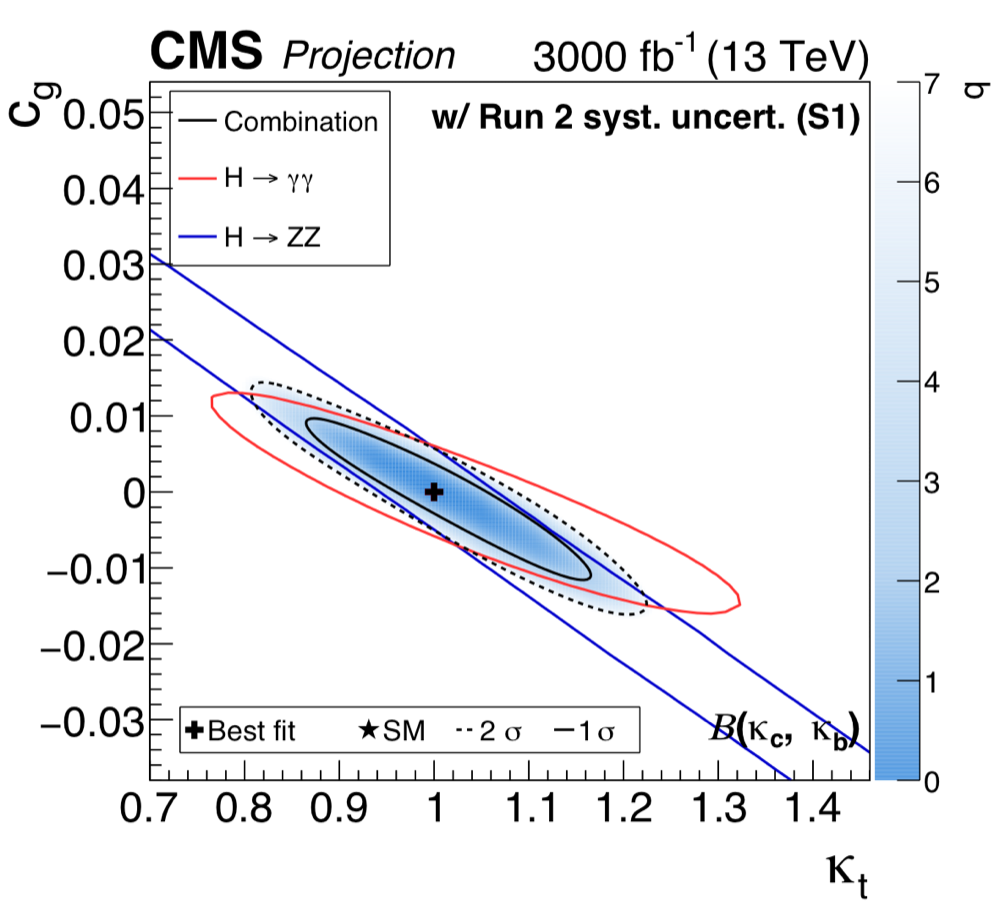
\includegraphics[width=0.49\linewidth]{\main/section2/plots/differentials/projection_ktcg_plot_couplingdependentBRs.png}
    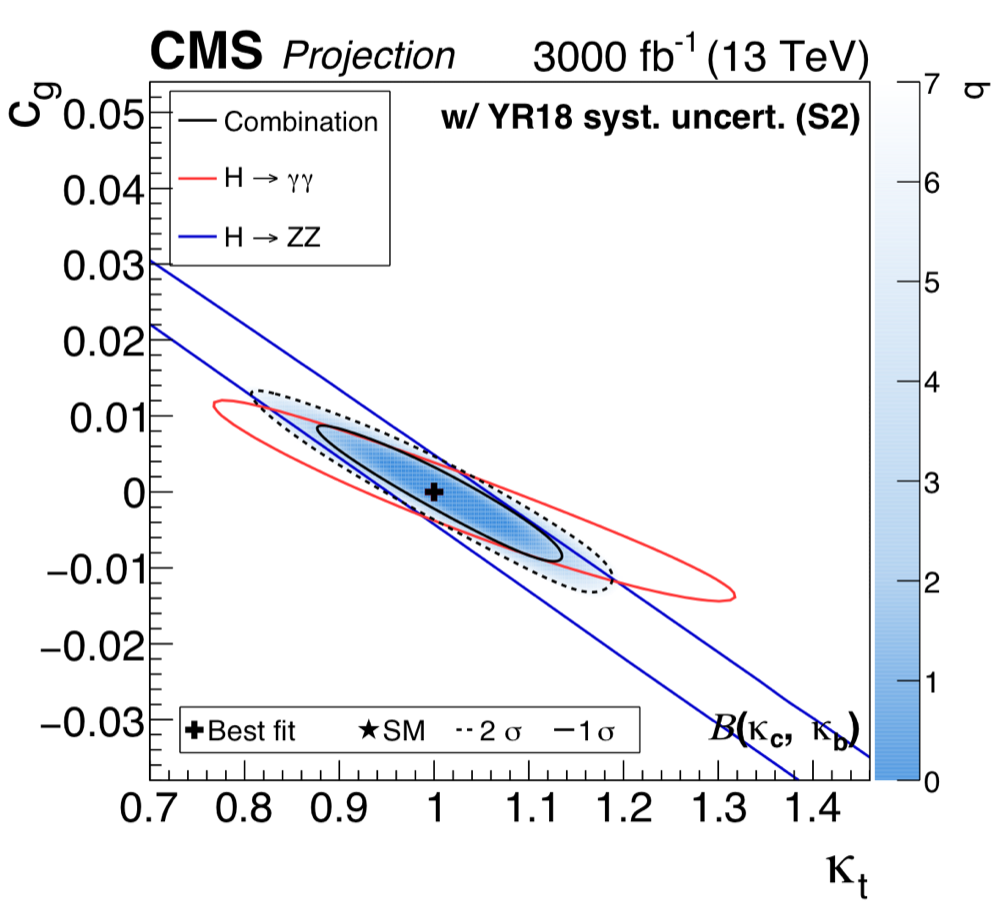
\includegraphics[width=0.49\linewidth]{\main/section2/plots/differentials/projection_ktcg_plot_couplingdependentBRs_scenario2.png}
    % 
    \caption{
        Projected simultaneous fit for $\kappat$ and $\cg$, assuming a coupling dependence of the branching fractions for Scenario 1 (left) and Scenario 2 (right).
        % 
        The one standard deviation contour is drawn for the combination ($\hgg$, $\hzz$, and $\hbb$), the $\hgg$ channel, and the $\hzz$ channel in black, red, and blue, respectively.
        % 
        For the combination the two standard deviation contour is drawn as a black dashed line, and the shading indicates the negative log-likelihood, with the scale shown on the right hand side of the plots.
        }
    \label{fig:ktcg_couplingdependentBRs}
  \end{center}
\end{figure}

In order to determine solely the constraint obtained from the distribution (and not the overall normalisation), the fit is repeated with the branching fractions implemented as nuisance parameters with no prior constraint, effectively profiling the overall normalisation.
% 
With this parametrisation, the sensitivity to the sign of $\kappat$ coming from the $\hgg$ branching fraction is lost.
% 
The fits obtained this way are shown in Fig.~\ref{fig:ktcg_floatingBRs}; although less significantly, the loop is still distinguished from the point-like coupling to the gluon field, using only the information in the shape of the distribution.

\begin{figure}[hbtp]
  \begin{center}
    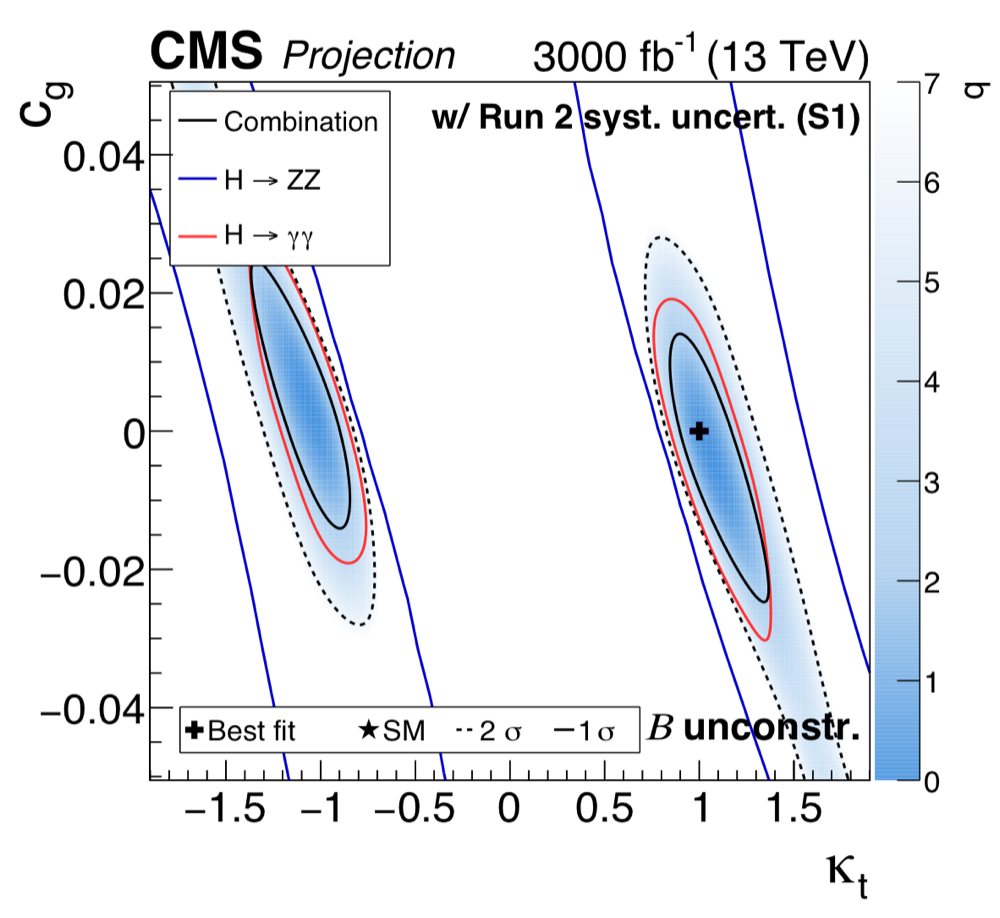
\includegraphics[width=0.49\linewidth]{\main/section2/plots/differentials/projection_ktcg_plot_floatingBRs.png}
    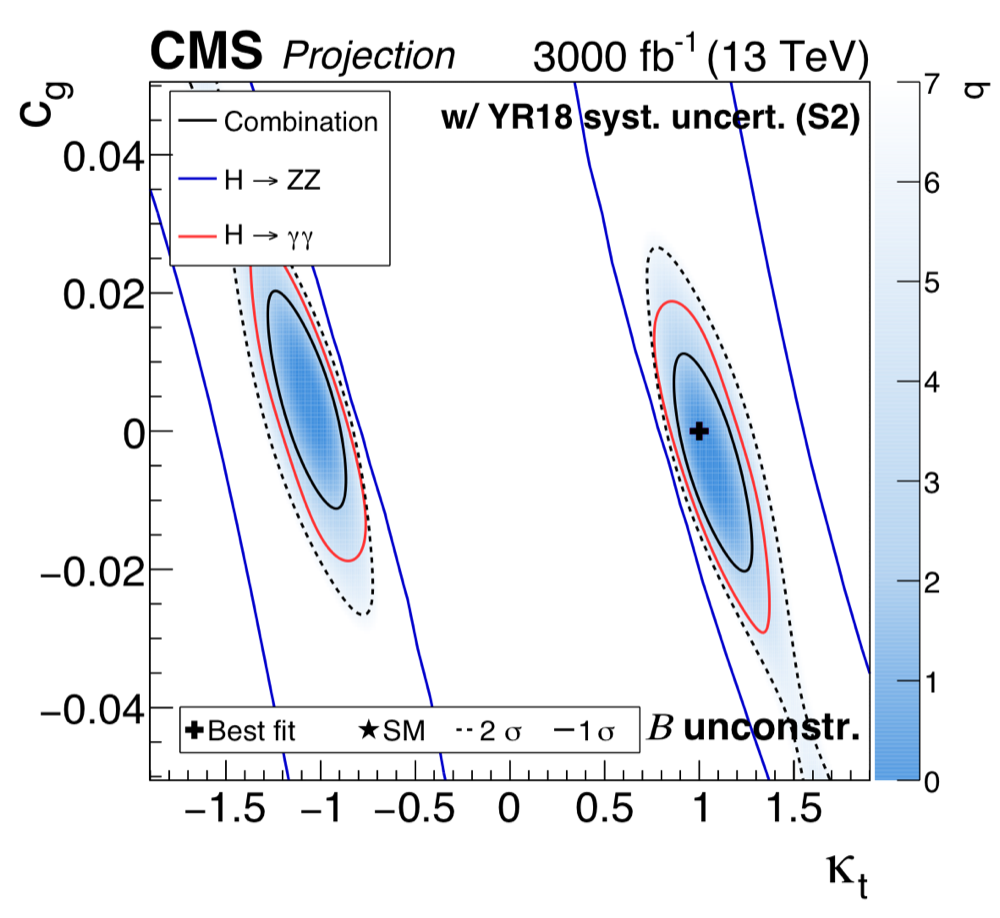
\includegraphics[width=0.49\linewidth]{\main/section2/plots/differentials/projection_ktcg_plot_floatingBRs_scenario2.png}
    % 
    \caption{
        Projected simultaneous fit for $\kappat$ and $\cg$ with the branching fractions implemented as nuisance parameters with no prior constraint for Scenario 1 (left) and Scenario 2 (right).
        % 
        The one standard deviation contour is drawn for the combination ($\hgg$, $\hzz$, and $\hbb$), the $\hgg$ channel, and the $\hzz$ channel in black, red, and blue, respectively.
        % 
        For the combination the two standard deviation contour is drawn as a black dashed line, and the shading indicates the negative log-likelihood, with the scale shown on the right hand side of the plots.
        }
    \label{fig:ktcg_floatingBRs}
  \end{center}
\end{figure}




